% Persoonlijk verslag van TinLab AA
% Mathematical Symbols:
% https://oeis.org/wiki/List_of_LaTeX_mathematical_symbols
\documentclass{article}% article report slides book letter beamer memoir minimal proc 
\usepackage{graphicx}
\usepackage{verbatim}% for multi line comments
\usepackage[dutch]{babel}
\usepackage{gensymb}% graden teken
\usepackage{multicol}
\begin{document}
\sffamily
\begin{titlepage}
  \centering
    \vfill
    {\bfseries\Huge
      Verslag Tinlab Advanced Algorithms \\
        \vskip2cm
      }
      {\bfseries\Large
        J. I. Weverink\\
      }
      {
        \bfseries\normalsize
        \ldots\\
        \vskip1cm
        \today\\
    }    
    \vfill
    
\includegraphics[width=4cm]{pictures/logohr.png} % also works with logo.pdf
    \vfill
    \vfill
\end{titlepage}
\newpage
\tableofcontents

\newpage
\section{Inleiding}
Zie hier een referentie naar Royce~\cite{royce1987managing} en nog een naar Clarke~\cite{modelchecking}\ldots 




\clearpage %========================================================================




\section{Requirements}

\subsection{Requirements}
% Wat zijn requirements?
% behoefte of noodzaak
Requirements zijn beschrijvingen over hoe een product zou moeten functioneren. Zo verandert de betekenis van een requirement als de machine in een andere omgeving wordt geplaats. De requirements voor de verwaring van een ruimte bijvoorbeeld: Binnen moet het altijd warm zijn. In nederland kunnen we zeggen dat 25$^{\circ}$C als warm wordt aangezien. Terwijl op de noordpool dat op een lager punt zal zijn.

Anders gezegd zijn requirements geen harde eisen. Dit komt doordat de requirements zijn geformuleerd van het perspectief van de opdrachtgever. De opdrachtgever kan de requirtements geven zonder kennis te hebben van de machine die het moet gaan uitvoeren. De requirements die zijn opgesteld geven dan ook geen grenzen aan die overscheden kunnen worden.

% system requirements software requirements 
Onder requirements zijn er verschillende soorten requirements. Zo zijn system requirements opgesteld voor het hele systeem en bevatten subsystemen die die kunnen bestaan uit software en hardware. Hier moet uiteindelijk alles ervoor zorgen dat deze requirement wordt gehaald. Software requirement zijn niet bedoeld voor het hele systeem, maar behappen alleen de de software van het systeem. Software requirement zijn niet bedoeld voor het hele systeem, maar behappen alleen de software van het systeem. De software requirements kunnen gaan over over de functionele eisen, gebruikers eisen en zakelijke vereisten.
%software requirements: https://books.google.nl/books?hl=nl&lr=&id=nbpCAwAAQBAJ&oi=fnd&pg=PT32&dq=what+are+software+requirements&ots=9pK_H20xTk&sig=tEhuqR8M3pOWPPM4kDu4yOSfOys&redir_esc=y#v=onepage&q=what%20are%20software%20requirements&f=false
Requirements zijn onder te verdelen in verschillende delen: 
\begin{multicols}{2}
\begin{itemize}
\item Functional Requirement
\item Performance requirement
\item Usability requirement
\item User requirement
\item Interface requirement
\item Modes requirement
\item Adaptability requirement
\item Physical requirement
\item Design requirement
\item Enviromental requirement
\item Logistical requirement
\end{itemize}
\end{multicols}

%	https://www.sebokwiki.org/wiki/System_Requirements#Definition_and_Purpose_of_Requirements
% Hoe krijgt men requirements
% Wat voor requirements elication technieken zijn er zoal?
% 	functional, performance, constraint
% Wat is het verschil tussen functionelen en non--functionelen requirements?
Onder deze verschillende requirements zijn er nog twee soorten, functionele en niet-functionele requirements. 
Functionele requirements geven aan wat het systeem moet doen en kunnen. Niet-functionele requirements geven de eigenschappen aan van het systeem, zoals snelheid, veiligheid en bruikbaarheid. Met andere woorden functionele requirements geven informatie over het "wat". niet-functionele requirements geven informatie over het "hoe".

% wat is mode confusion?
\subsubsection{Mode confusion}
De naam van het begrip zegt het eigenlijk allemaal. Bij mode confusion maakt de gebruiker een vergissing in de huidige of geactiveerde modus van het systeem. De gebruiker denk dat het systeem in modus A staat terwijl het werkelijk in modus B staat. 
%	mode van een apparaat bijv. auto in sport en eco modus

% Wat verstaat men onder automatiseringparadox
\subsubsection{Automatisering paradox}
Automatiseringsparadox. Wanneer een systeem is dat volledig geautomatiseerd moet worden is er altijd een wel een stap die dat nog niet is. Wanneer er een stap is geautomatiseerd moet er weer iets anders geautomatiseerd worden, om het hele systeem automatisch te krijgen.

\subsection{specificaties}
%system specifications	software specifications
Specificaties zijn eigenlijk niet heel veel anders dan requirements. ze beschrijven beide een systeem of een deelsysteem. Het grote verschil tussen de twee is de grenzen die ze opleggen. Bij requirements is er ruimte voor interpetatie, bij specificaties is die ruimte voor interpetatie er niet.

De specificaties geven geen ruimte voor interpetatie, omdat ze 'meetbare' informatie bevatten. In specificaties worden meetbare eenheden gebruikt, zoals 10 meter of 10$^{\circ}$C. Door dat de eisen een meetbare eenheid bevatten kan hiervan niet worden afgewezen. Deze specificaties zullen dan ook niet veranderen als het wordt gebruikt in een ander land, doordat de eenheden zijn gegeven.
\\

Stel we nemen het eerder genoemde requirement voorbeeld: "Binnen moet het altijd warm zijn." Als we dit vertalen naar een specificatie wordt het: "Binnen moet het altijd minimaal 20$^{\circ}$C zijn."




\clearpage %========================================================================




\subsection{Het vier variabelen model}
% Het 6 variable model
%\hspace*{2cm}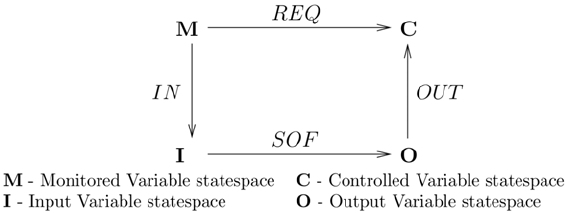
\includegraphics[width=10cm]{pictures/4_var_model.png}
%\cite{variabelmodel}
% source https://www.researchgate.net/figure/4-Variable-Model-of-Parnas-Madey_fig3_270733268

\subsubsection{Monitored variabelen}
Monitored variabelen zijn waarnemingen die kunnen worden gemeten vanuit de omgeving. De waarnemingen worden gemeten door sensoren, de gemeten data wordt als input gebruikt. Voorbeelden van zulke waarnemingen zijn:
\begin{itemize}
  \item Temperatuur
  \item Licht intensiteit
  \item Luchtvochtigheid
  %\item Wat je allemaal met sensoren kunt meten
\end{itemize}

\subsubsection{Controlled variabelen}
Controlled variablen zijn waarnemingen die in zekere zin beïnvloed kunnen worden. Zo kunnen de controlled variabelen 'bestuurd' worden, er is controle over.Voorbeelden van controleerbare waarnemingen zijn:
\begin{itemize}
  \item Temperatuur
  \item Licht intensiteit
  %\item Wat je allemaal kan beinvloeden
\end{itemize}

\subsubsection{Input variabelen}
Input variablen zijn de waardes, of de data, die een sensor doorstuurt naar de software die het systeem bestuurd. Deze data staat voor de waardes die de sensor heeft gemeten vanuit de omgeving. Omdat de sensor de gemeten waardes heeft omgezet in data kan dit worden gebruikt in de software, om bijvoordbeeld berekeningen mee te maken.

\subsubsection{Output variabelen}
Output variabelen zijn de 'uitkomsten' van de software die worden uitgelezen door de actuatoren. De actuatoren handelen aan de hand van de output van de software.

\subsection{Rampen}

\subsubsection{Therac-25}
\begin{description}
\item[Beschrijving]
\item[Datum en plaats] 
\item[Oorzaak]
  %Beschrijf wat er mis ging in termen van het vier variabelen model/requirements/specificaties
\end{description}

\subsubsection{Vlucht 1951}

\subsubsection{Tsjernobyl 1986}

\subsubsection{Ethiopian Airlines 302}

\subsubsection{Ramp 5}
\subsubsection{Ramp 6}




\clearpage %========================================================================




\section{Modellen}
Een model is een schematische weergaven van de werking van een systeem. Elk soort systeem kan gemodelleerd worden. of het ingewikkeld of heel simpel is. Een model wordt altijd zo realistisch mogelijk gemaakt. Dat wil zeggen dat de belangrijke onderdelen in het model ook terug komen het "'echte"' systeem.
\begin{comment}
********** NOTES **********\\
Een goed model heeft een duidelijk object dat gemodelleerd moet worden, er is duidelijk \textbf{wat} er beschreven moet worden.
\\
Een goed model heeft een duidelijk doel.
-waarom modelleren we? (voor communicatie of verificatie, analyse, etc.)
\\
Een goed model is traceerbaar: elk onderdeel is te herleiden tot de onderdelen van het "echte"systeem.
\\
Een goed model is waarheidsgetrouw: relevante onderdelen van het model komen terug in de werkelijkheid.
\\
een goed model is eenvoudig, maar niet te eenvoudig
\\
Een goed model is uitbreidbaar en herbruikbaar: in de toekomst is het eenvoudig verder te werken met dit model en kunnen zelfs \textit{klassen} van vergelijkbare  systemen gemaakt worden
\\
Een goed model deelt geen jargon/semantiek met andere documenten en modellen.
\\\\
Richtlijnen (tegenstrijdig heden:
\\
Waarheidgetrouw vs simpelheid
duidelijheid vs. gedeeld jargon/semantiek
\end{comment}
\subsection{De Kripke structuur}
Een kripke structuur bestaat uit binaire overgangsrelaties tussen state, die de werking van een systeem weergeven.\cite{kripkestructure} Aan deze overgangen en handelingen kunnen eigenschappen gekoppeld worden. Op deze manier kunnen de handelingen en eigenschappen gecontroleerd en verifieerd worden en het systeem getest worden of het op juiste wieze handelt. De acties binnen een kripke structuur lopen altijd synchroon.


\subsection{Soorten modellen} %sir model
Andere soorten modellen zijn discrete and continuous -time Markov chains, deze zogehete "'Marko chains"' zijn een vorm van stochastic model checking. Bovendien kosten continuous chains enorm veel kracht om te berekenen. Zoals A. Philippe en C. Robert het verwoorden in hun boek \textit{Linking Discrete and Continuous Chains}\cite{linkingchains} hebben deze vormen een gebrek aan intuïtieve basis achter de theorie van Markov chains.

% Winskel Model
% SIR Model




\subsection{Tijd}
Tijd kan een belangrijke rol spelen in het modelleren van een systeem. De tijd die jij en ik bijhouden op een 24-uurs klok die is net zo van invloed op een systeem. De handellingen gebeuren immers in de loop van de tijd.
In UPPAAL kan met het verloop van tijd ook gewerkt worden. De tijd verloop is altijd synchroon. Dit houdt in dat er geen 2 of meerdere acties tegelijk uitgevoerd kunnen worden.

%MEER TEXT






\subsection{Guards en invarianten}
Guards zijn voorwaarden waaraan moet worden voldaan voordat een transitie genomen kan worden. Het is als het ware een "if statement", is de uitkomst niet true dan kan de transitie niet genomen worden.

% invariant [https://link.springer.com/chapter/10.1007/978-88-470-2107-5_4]
Invariant theory is al heel oud en komt oorspronkelijk uit de wiskunde. Over de jaren heen heeft het verschillende betekenissen gekregen. Hermann Weyl legt dit uitgebreid uit in zijn boek \textit{The Classical Groups}. \cite{classicalgroups} G. Rota haal uit het boek van Weyl 2 beweringen. De eerste "all geometric facts are expressed by the vanishing of invariants". en de tweede "all invariants are invariants of tensors". Echter denk ik dat deze beweringen niet van toepassing zijn in deze context.

In de context van de opdracht zijn invarianten voorwaarden die kunnen worden vastgesteld aan een state. De state moet worden verlaten zodra de invariant niet meer van kracht is(als de voorwaarde niet meer behaald is) en zal geforceerd worden een beschikbare transitie te nemen.

\subsection{Deadlock}
Een deadlock ontstaat als er een proces in groep processen een geheugen locatie bezet houden en bij een andere geheugen locatie wilt komen, maar deze wordt al bezet gehouden door een ander proces in de groep. Dit is een deadlock in de ogen van een programmeur.\cite{deadlockproblem}

Een deadlock heeft echter een hele andere definitie als het neerkomt op modelleren. In de wereld van modelleren heeft een deadlock niets te maken met gebruik van geheugen locaties. Een deadlock kan alleen ontstaan als er ristricties zijn gelegd aan transities. Deze restricties zorgen ervoor dat niet elke transitie altijd genomen kan worden. Als er een state is waar geen volgende transitie meer mogelijk is preken we van een deadlock.

\subsection{Zeno gedrag}
Zeno gedrag is een wiskundige term. het beschrijft een situatie waarin in een bepaalde tijd oneindig veel transities ontstaan.\cite{sufficientconditions} Doordat er oneindig veel stappen worden gezet in een korte (of lange) tijd, moeten de stappen extreem klein zijn. Dat moet wel want er is immers geen einde aan te krijgen. 




\clearpage %========================================================================




\section{Logica}
Logica is een de wetenschap die focussed op de regels van redeneren.
\subsection{Propositielogica}
Een propositie is een taaluiting ofwel een bewering of uitspraak uitgedrukt in een zin. De zin beschrijft een situatie of stand van zaken. 
Deze zin heeft een waarheidswaarde van 0 (nietwaar) of 1 (waar), het kan absoluut niet beide zijn. Bijv. "'De auto staat stil."' of 

In de propositielogica worden deze proposities gebruik is samenwerking met logische operatoren zoals bijv. AND en OR.\cite{propositionlogic}

\subsection{Predicatenlogica}
Een predicaat is een eigenschap of kwaliteit dat over iets gezegd gezegd kan worden. Door gebruik te maken van predicatenlogica kan een zin met een predicaat vertaald worden op een dusdanige manier dat een (computer) systeem dit kan begrijpen.
Het predicaat wordt vertaald naar een wiskundige formule. In deze formule zijn alle eigenschappen en relaties nogsteeds zichtbaar.

\subsection{Kwantoren}
Met kwantoren worden eigenschappen gekoppeld aan een onderwerp waarover zei informatie verschaffen. Stel de volgende kwantoren over rotten appels in een winkel
Een voorbeeld hiervan is:
\begin{description}
\item $\exists$xP(x): Er zijn appels die rot zijn.
\item $\forall$xP(x): Alle appels zijn verrot.
\end{description}
Als we in deze kwantoren stellen dat P staat voor verrot en de x voor appels dan zijn de beweringen die erachter staan van kracht.


\subsection{Dualiteiten}
Dualiteit betekend dat van een stelling er een andere stelling bestaat met dezelfde betekenis.
\begin{center}
$\neg\forall$xP(x): $\exists$x$\neg$P(x)
\end{center}

Als we weer het voorbeeld van de appels nemen staat hier effectief links niet alle appels zijn verrot. Aan de rechter kant staat Er zijn appels die niet verrot zijn.
% presentatie 03-15

\section{Computation tree logic}
\begin{comment}
Computation tree logic (CTL) is a branching-time logic, meaning that its model of time is a tree-like structure in which the future is not determined; there are different paths in the future, any one of which might be an actual path that is realized. It is used in formal verification of software or hardware artifacts, typically by software applications known as model checkers, which determine if a given artifact possesses safety or liveness properties. For example, CTL can specify that when some initial condition is satisfied (e.g., all program variables are positive or no cars on a highway straddle two lanes), then all possible executions of a program avoid some undesirable condition (e.g., dividing a number by zero or two cars colliding on a highway). In this example, the safety property could be verified by a model checker that explores all possible transitions out of program states satisfying the initial condition and ensures that all such executions satisfy the property. Computation tree logic belongs to a class of temporal logics that includes linear temporal logic (LTL). Although there are properties expressible only in CTL and properties expressible only in LTL, all properties expressible in either logic can also be expressed in CTL*.
\end{comment}

\subsection{De computation tree}
Computation tree logic is een model waar de tijd een vertakkings structuur aan states heeft, waarin de toekomst nog onbepaald is. Er zijn verschillende wegen die afgelegd kunnen worden, waarvan er één mogelijk werkelijk genomen zal worden.

Een computation tree wordt opgebouwd vanuit de begin state. vervolgens komt er nog een laag aan de hand van alle transities die deze begin state kan nemen. De tweede laag bestaat dan uit alle states waar de transities van de begin state eindigen. Dit kan doorgaan tot er state tegen komt waar geen volgende transitie uit te volgen is.

\subsection{Operator: AG}
De betekenis van AG is makkelijk te onthouden A = Always, G = Globally. Dit houdt in dat het niet uit maakt waar je bent, je zal altijd van welke positie dan ook bij een gedefinieerde state uitkomen.

\subsection{Operator: EG}
De EG operator staat voor ''Exists Globally"'. Dit betekent dat er van alle wegen een aantal zijn, niet allemaal, die leiden naar het gedefinieerde state. 

\subsection{Operator: AF}
De AF operator kan worden samengevat als "'Always Evetually"'. Dit kan worden vertaald naar het niet uit welke weg wordt genomen, er is altijd een moment waarop het gedefinieerde state is bereikt.

\subsection{Operator: EF}
De EF lijkt uiteraard op de AF operatoo, alleen geld bij de EF operator dat \textbf{niet} bij alle wegen de gedefiniëerde state wordt bereikt. Met andere woorden op enkele wegen zal er uiteindelijk de gedefiniëerde state worden bereik. Deze operator kan dan ook worden samen gevat als "'Exists Eventually"'.

\subsection{Operator: AX}
De AX operator is anders dan de vorigen operatoren. Het heeft namelijk alleen maar betrekking tot de volgende state. De AX operator kan worden samengevat als "'Always Next"', wat dus inhoud at dus elk volgende state de gedefinieerde state zal bevatten.

\subsection{Operator: EX}
Het spreekt voor zich dat de EX operator ook alleen voor de volgende state zal gelden. De EX operator staat dan voor "'Exists Next"'. Voor de EX operator geld dat er in enkele volgende states de gewenste state bereikt zal zijn.

\subsection{Operator: p U q}
Bij deze operator draait het vooral om de U. De U kan worden verstaan als "'Until"', zo staat er hier p is waar tot dat q waar is. Anders gezegd is p waar en ophet moment dat dat stopt, p onwaar wordt, dan wordt q waar. Het is moeglijk voor p en q om uiteindelijk beide onwaar te worden, maar dit gebreurt pas nadat de "'cyclus"' van p naar q minimaal één keer is doorlopen.

Een raar maar simpel voorbeeld hiervan zou zijn een doos die wordt getild door persoon p, p is waar. Na enige tijd laat persoon p de doos vallen, die de doos wordt gevangen door persoon q. Op dit moment word q waar en p onwaar. Het komt dus niet voor dat de p en q samen waar zijn.

Deze operator kan genest worden in een Always of Exist operator. Door dit te doen komt er het volgende uit:
\\
A(p U q): Voor deze samenstelling geld dat op alle wegen de p U q operator van kracht is.
\\
E(p U q): Hier geld dat op enkele wegen de p U q operator van kracht is.

\subsection{Operator: p R q}
De R operator is zeer gelijk aan de U operator. Ze bevatten beiden de eigenschap dat nadat p niet meer waar is dat q waar is. Er is een eigenschap die echter het verschil maakt. De R operator heeft een moment, een state, waarin zowel p als q waar zijn.

Om dit in hetzelfde voorbeeld te verduidelijken. Draagt persoon p nu weer de door, p is waar. Zodra persoon p moe wordt geeft hij de doos over aan persoon q. Let op dat tijdens het geven van de doos er een moment is waarin zowel persoon p als q de doos vasthebben. Dit is het verschil met de U operator, er is een state waarin beide p en q waar zijn.

Net als de U operator is de R operator ok te nestelen in de Always en de Exists operatoren. Hieruit volgt:
\\
A(p R q): Voor deze samenstelling geld dat op alle wegen de p R q operator van kracht is.
\\
E(p R q): Hier geld dat op enkele wegen de p R q operator van kracht is.



\subsection{Fairness}
De letterlijke vertaling van fairness is eerlijkheid. Dat is ook een beetje waar de fairness die hier wordt edoeld op slaat. Fairness betekent namelijk dat alle taken in een systeem "'aandacht"' zullen krijgen. De zogeheten aandacht wordt eerlijk verdeeld.

Als we fairness uitdrukken in operatoren dan komen we uit op AG(AF(p)). Als wij stellen de p staat voor aandacht aan een process. Dan staat hier nu dat het niet uit maakt welke transitie route we aflegen uiteindelijk zal het process aandacht krijgen, zelfs als het al een keer aandacht heeft gehad. het is dus in feite een loop.
%elke taak krijgt aandacht en als die dat heeft gehad zal hij het vaker krijgen

\subsection{Liveness}
Wat gezegd zou kunnen worden over liveness is dat het een vorm van fairness is. Dit komt door dat de operator schrijfwijze  vrijwel gelijk is aan die van fairness. liveness wordt geschreven als AG(r $\rightarrow$ AF(p)), wat lijk op fairness AG(AF(p)). Wat "'extra"' is bij liveness is de r $\rightarrow$ genesteld in de AG. De pijl kan worden gezien als een if-statement, if r = true dan AF, met de r als de bepalende factor. Als de r waar is dan is er een geval van welke weg, of transitie, we ook nemen daar komen we vroeg of laat in een state waar p geld.

Zoals in het artikel van B. Alpern en B. Schneider\cite{definingliveness} wordt gezegd is kan liveness voorkomen in 3 vormen starvation freedom, termination en guarenteed service. Dez vormen zijn ook weer terug te vinden in het boek \textit{Synchronization Algorithms ans concurrent Programming}\cite{synchronizationalgorithms} van G. Taubenfeld





\clearpage  %========================================================================




\bibliography{references} % DIT ZIJN VOORBEELDEN

\begin{thebibliography}{9}

\bibliography{refrences}
\bibitem{variabelmodel} 
Knuth: Use of Tabular Expressions for Refinement Automation,
\\\texttt{https://www.researchgate.net/figure/4-Variable-Model-of-Parnas-Madey\_fig3\_270733268}
%https://www-fourier.ujf-grenoble.fr/~panchish/ETE%20LAMA%202018-AP/Weyl_The%20Classical%20Groups.pdf
\bibitem{classicalgroups} 
WEYL, H (1966).
\textit{The Classical Groups: Their Invariants and Representations.}.\\ 
PRINCETON, NEW JERSEY: Princeton University Press.

\bibitem{kripkestructure} 
V. Gupta, V Pratt (1993)
\textit{Concurrent Kripke Structures}. 
Stanford University.

\bibitem{stochasticmodel} 
Kwiatkowska M., Norman G., Parker D. (2007)
\textit{Stochastic Model Checking}. 
Bernardo M., Hillston J. Springer, Berlin, Heidelberg.

\bibitem{linkingchains} 
Philippe A., Robert C.P. (1998)  
\textit{Linking Discrete and Continuous Chains}. 
Robert, Christian P., Springer, New York, NY.

\bibitem{propositionlogic}
H. K. Büning, T. Lettman (1999).
\textit{Proposition logic: deduction an algorithms}\\
Cambridge university press, Cambridge. 

\bibitem{synchronizationalgorithms}
G. Taubefeld (2006).
\textit{Synchronization Algorithms and Concurrent Programming}\\
Pearson Education Limited, Edinburgh. 

\bibitem{deadlockproblem} 
S. Isloor, T. Anthony Marsland (1980)
\textit{The Deadlock Problem: An Overview}. 
% geen publisher

\bibitem{sufficientconditions}
A. D. Ames, A. Abate and S. Sastry (2005)
\textit{Sufficient Conditions for the Existence of Zeno Behavior}.
University of Californioa, Berkeley.

\bibitem{definingliveness} 
B. Alpern, F. B. Schneider (1985)
\textit{Defining Liveness}. 
% geen publisher

\bibitem{latexcompanion} 
Michel Goossens, Frank Mittelbach, and Alexander Samarin. 
\textit{The \LaTeX\ Companion}. 
Addison-Wesley, Reading, Massachusetts, 1993.

\bibitem{rota} 
Rota G. -C. (2001).
\textit{Algebraic Combinatorics and Computer Science: A Tribute to Gian-Carlo Rota}.
Crapo, H. and Senato, D., Springer Milan.

\bibitem{einstein} 
Albert Einstein. 
\textit{Zur Elektrodynamik bewegter K{\"o}rper}. (German) 
[\textit{On the electrodynamics of moving bodies}]. 
Annalen der Physik, 322(10):891–921, 1905.

\bibitem{knuthwebsite} 
Knuth: Computers and Typesetting,
\\\texttt{http://www-cs-faculty.stanford.edu/\~{}uno/abcde.html}

\end{thebibliography}

\end{document}


book:
\bibitem{}
author (release year).
\textit{title}\\
Editors., Publisher. 


What is a good model? Artikel F. Vaandrager

What is a model? E griffiths
